\documentclass[10pt]{article}
\usepackage{tikz}
\usetikzlibrary{shapes.misc}
\usepackage[margin=0cm]{geometry}
\pagestyle{empty}
\tikzstyle{every node}=[cross out, draw, red]

\begin{document}

\vspace*{\fill}
\begin{center}
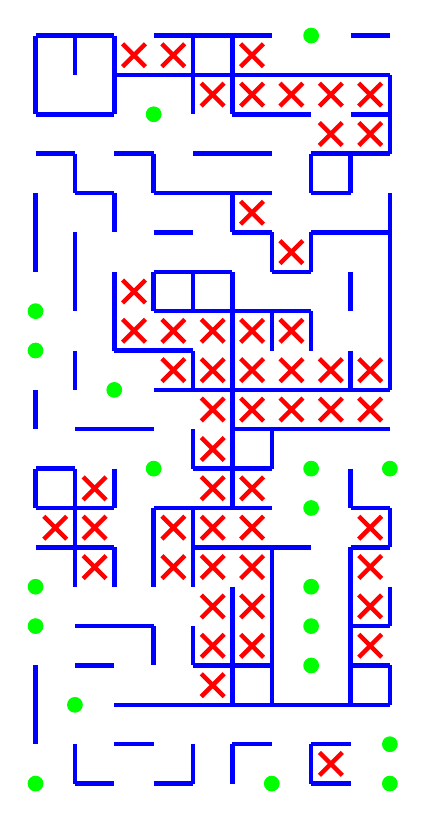
\begin{tikzpicture}[x=0.5cm, y=-0.5cm, ultra thick, blue]
% Walls
    \draw (0,0) -- (2,0);
    \draw (3,0) -- (6,0);
    \draw (8,0) -- (9,0);
    \draw (2,1) -- (9,1);
    \draw (0,2) -- (2,2);
    \draw (5,2) -- (7,2);
    \draw (8,2) -- (9,2);
    \draw (0,3) -- (1,3);
    \draw (2,3) -- (3,3);
    \draw (4,3) -- (6,3);
    \draw (7,3) -- (9,3);
    \draw (1,4) -- (2,4);
    \draw (3,4) -- (6,4);
    \draw (7,4) -- (8,4);
    \draw (3,5) -- (4,5);
    \draw (5,5) -- (6,5);
    \draw (7,5) -- (9,5);
    \draw (3,6) -- (5,6);
    \draw (6,6) -- (7,6);
    \draw (3,7) -- (7,7);
    \draw (2,8) -- (4,8);
    \draw (3,9) -- (9,9);
    \draw (1,10) -- (3,10);
    \draw (5,10) -- (9,10);
    \draw (0,11) -- (1,11);
    \draw (4,11) -- (6,11);
    \draw (0,12) -- (2,12);
    \draw (3,12) -- (6,12);
    \draw (8,12) -- (9,12);
    \draw (0,13) -- (2,13);
    \draw (4,13) -- (7,13);
    \draw (8,13) -- (9,13);
    \draw (1,15) -- (3,15);
    \draw (8,15) -- (9,15);
    \draw (1,16) -- (2,16);
    \draw (4,16) -- (6,16);
    \draw (8,16) -- (9,16);
    \draw (2,17) -- (9,17);
    \draw (2,18) -- (3,18);
    \draw (5,18) -- (6,18);
    \draw (7,18) -- (8,18);
    \draw (1,19) -- (2,19);
    \draw (3,19) -- (4,19);
    \draw (7,19) -- (8,19);
    \draw (0,0) -- (0,2);
    \draw (0,4) -- (0,6);
    \draw (0,9) -- (0,10);
    \draw (0,11) -- (0,12);
    \draw (0,16) -- (0,18);
    \draw (1,0) -- (1,1);
    \draw (1,3) -- (1,4);
    \draw (1,5) -- (1,7);
    \draw (1,8) -- (1,9);
    \draw (1,11) -- (1,14);
    \draw (1,18) -- (1,19);
    \draw (2,0) -- (2,2);
    \draw (2,4) -- (2,5);
    \draw (2,6) -- (2,8);
    \draw (2,11) -- (2,12);
    \draw (2,13) -- (2,14);
    \draw (3,3) -- (3,4);
    \draw (3,6) -- (3,7);
    \draw (3,12) -- (3,14);
    \draw (3,15) -- (3,16);
    \draw (4,0) -- (4,2);
    \draw (4,6) -- (4,7);
    \draw (4,8) -- (4,9);
    \draw (4,10) -- (4,11);
    \draw (4,12) -- (4,14);
    \draw (4,15) -- (4,16);
    \draw (4,18) -- (4,19);
    \draw (5,0) -- (5,2);
    \draw (5,4) -- (5,5);
    \draw (5,6) -- (5,12);
    \draw (5,14) -- (5,17);
    \draw (5,18) -- (5,19);
    \draw (6,5) -- (6,6);
    \draw (6,7) -- (6,8);
    \draw (6,10) -- (6,11);
    \draw (6,13) -- (6,17);
    \draw (7,3) -- (7,4);
    \draw (7,5) -- (7,6);
    \draw (7,7) -- (7,8);
    \draw (7,18) -- (7,19);
    \draw (8,3) -- (8,4);
    \draw (8,6) -- (8,7);
    \draw (8,8) -- (8,9);
    \draw (8,11) -- (8,12);
    \draw (8,13) -- (8,17);
    \draw (9,1) -- (9,3);
    \draw (9,4) -- (9,9);
    \draw (9,12) -- (9,13);
    \draw (9,14) -- (9,15);
    \draw (9,16) -- (9,17);
% Pillars
    \fill[green] (7,0) circle(0.2);
    \fill[green] (3,2) circle(0.2);
    \fill[green] (0,7) circle(0.2);
    \fill[green] (0,8) circle(0.2);
    \fill[green] (2,9) circle(0.2);
    \fill[green] (3,11) circle(0.2);
    \fill[green] (7,11) circle(0.2);
    \fill[green] (9,11) circle(0.2);
    \fill[green] (7,12) circle(0.2);
    \fill[green] (0,14) circle(0.2);
    \fill[green] (7,14) circle(0.2);
    \fill[green] (0,15) circle(0.2);
    \fill[green] (7,15) circle(0.2);
    \fill[green] (7,16) circle(0.2);
    \fill[green] (1,17) circle(0.2);
    \fill[green] (9,18) circle(0.2);
    \fill[green] (0,19) circle(0.2);
    \fill[green] (6,19) circle(0.2);
    \fill[green] (9,19) circle(0.2);
% Inner points in accessible cul-de-sacs
    \node at (2.5,0.5) {};
    \node at (3.5,0.5) {};
    \node at (5.5,0.5) {};
    \node at (4.5,1.5) {};
    \node at (5.5,1.5) {};
    \node at (6.5,1.5) {};
    \node at (7.5,1.5) {};
    \node at (8.5,1.5) {};
    \node at (7.5,2.5) {};
    \node at (8.5,2.5) {};
    \node at (5.5,4.5) {};
    \node at (6.5,5.5) {};
    \node at (2.5,6.5) {};
    \node at (2.5,7.5) {};
    \node at (3.5,7.5) {};
    \node at (4.5,7.5) {};
    \node at (5.5,7.5) {};
    \node at (6.5,7.5) {};
    \node at (3.5,8.5) {};
    \node at (4.5,8.5) {};
    \node at (5.5,8.5) {};
    \node at (6.5,8.5) {};
    \node at (7.5,8.5) {};
    \node at (8.5,8.5) {};
    \node at (4.5,9.5) {};
    \node at (5.5,9.5) {};
    \node at (6.5,9.5) {};
    \node at (7.5,9.5) {};
    \node at (8.5,9.5) {};
    \node at (4.5,10.5) {};
    \node at (1.5,11.5) {};
    \node at (4.5,11.5) {};
    \node at (5.5,11.5) {};
    \node at (0.5,12.5) {};
    \node at (1.5,12.5) {};
    \node at (3.5,12.5) {};
    \node at (4.5,12.5) {};
    \node at (5.5,12.5) {};
    \node at (8.5,12.5) {};
    \node at (1.5,13.5) {};
    \node at (3.5,13.5) {};
    \node at (4.5,13.5) {};
    \node at (5.5,13.5) {};
    \node at (8.5,13.5) {};
    \node at (4.5,14.5) {};
    \node at (5.5,14.5) {};
    \node at (8.5,14.5) {};
    \node at (4.5,15.5) {};
    \node at (5.5,15.5) {};
    \node at (8.5,15.5) {};
    \node at (4.5,16.5) {};
    \node at (7.5,18.5) {};
% Entry-exit paths without intersections
\end{tikzpicture}
\end{center}
\vspace*{\fill}

\end{document}
